% Setup and frequently used packages
\documentclass[12pt]{article}
\usepackage[a4paper, margin=1in]{geometry}
\usepackage[utf8]{inputenc}
\usepackage[T1]{fontenc}
\usepackage{parskip} % Remove indent of new paragraph
\usepackage{titling}
\usepackage{graphicx} % To include graphics such as pictures
\usepackage{amsmath}
\usepackage{caption} % Used to allow empty captions for figures

% Setup title/author/date
\title{Jax Controller Report}
\author{Group 128}
\date{}

% References
\usepackage{hyperref} % Correct formatting for urls in references
\usepackage[style=apa]{biblatex}
\addbibresource{references.bib}

% Header
\usepackage{fancyhdr}
\pagestyle{fancyplain}
\fancyhf{}
\lhead{\theauthor}
\chead{}
\rhead{\thepage}
\renewcommand{\headrulewidth}{0.4pt}
\renewcommand{\plainheadrulewidth}{0.4pt}


\begin{document}
\maketitle

\section*{Bathtub Plant - Classic Controller}

\begin{tabular}{|l|l|}
\hline
\textbf{Parameter}   & \textbf{Value}\\ \hline
Epochs               & 50            \\ \hline
Timesteps            & 50            \\ \hline
Learning Rate        & 0.01          \\ \hline
Disturbance Range    & (-0.05, 0.05) \\ \hline
Initial $K_p$           & 0.1           \\ \hline
Initial $K_i$           & 0.1           \\ \hline
Initial $K_d$           & 0.1           \\ \hline
A                    & 10            \\ \hline
C                    & 0.1           \\ \hline
Initial Height Water & 5             \\ \hline
\end{tabular}

\begin{center}
    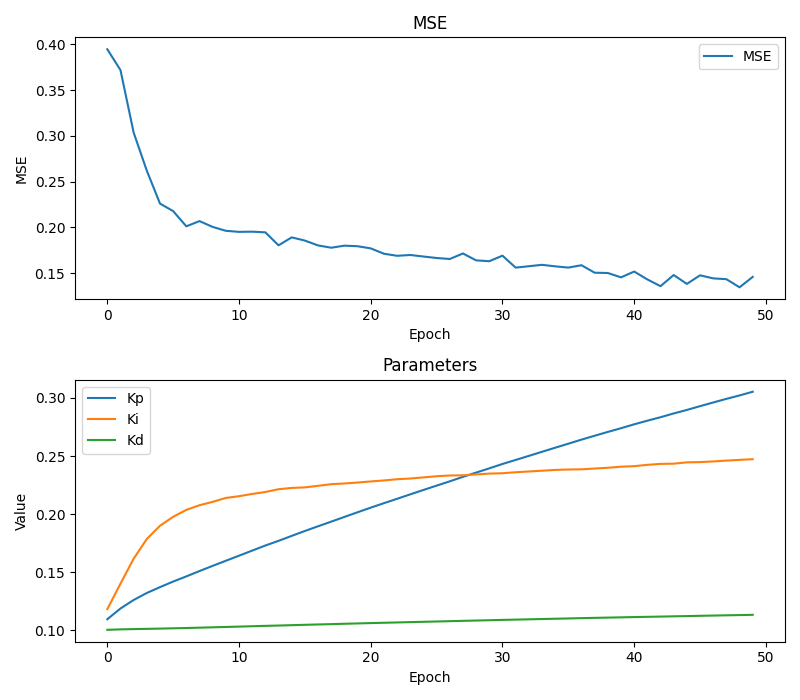
\includegraphics[width=0.8\linewidth]{figures/bathtub-classic.png}
\end{center}

The initial error is not that high but it quickly goes down within the first 10 epochs. After that it continues
to go down, but at a lower rate. Given more epochs it might go down further. The MSE varies but this might be a response
to the relatively high disturbance range. The parameters change more in the earlier epochs, especially the $K_i$. After about
10 epochs the $K_i$ parameter changes at a lower rate. This is probably reflected in the MSE plot after 10 epochs, as we
can see that the rate of change is lower after that point.

\section*{Bathtub Plant - AI Controller}

\begin{tabular}{|l|l|}
    \hline
    \textbf{Parameter}   & \textbf{Value}\\ \hline
    Epochs               & 50            \\ \hline
    Timesteps            & 50            \\ \hline
    Learning Rate        & 0.001          \\ \hline
    Disturbance Range    & (-0.05, 0.05) \\ \hline
    Number of Hidden Layers           & 2           \\ \hline
    Neurons per Layer           & [64, 32]           \\ \hline
    Initial Weight/Bias Range           & (-0.001, 0.001)           \\ \hline
    Activation Function                    & sigmoid            \\ \hline
    A                    & 10           \\ \hline
    C & 0.1             \\ \hline
    Initial Height Water & 5             \\ \hline
\end{tabular}
    
\begin{center}
    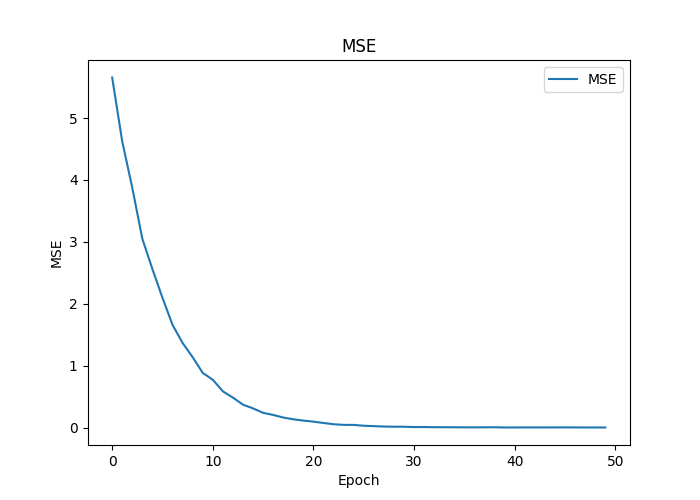
\includegraphics[width=0.8\linewidth]{figures/bathtub-ai.png}
\end{center}

In this run the initial error is higher. This might be because of the random initializing of weights and biases.
We can see that it goes steadily down, but the curve is not that steep. This is because the learning rate in this run is set
to 0.001 instead of 0.01 as in the run with the classic controller above. In particular we observed that the gradients for the
output layer could be high, indicating that these values were far off after initializing them. The controller still manages
to learn, and displays a considerate change in MSE.

\section*{Cournot Plant - Classic Controller}

\begin{tabular}{|l|l|}
    \hline
    \textbf{Parameter}   & \textbf{Value}\\ \hline
    Epochs               & 50            \\ \hline
    Timesteps            & 50            \\ \hline
    Learning Rate        & 0.01          \\ \hline
    Disturbance Range    & (-0.02, 0.02) \\ \hline
    Initial $K_p$           & 0.1           \\ \hline
    Initial $K_i$           & 0.1           \\ \hline
    Initial $K_d$           & 0.1           \\ \hline
    Maximum Price                    & 3            \\ \hline
    Marginal Cost                    & 0.1           \\ \hline
    Target Profit & 0.55             \\ \hline
    Initial $q_1$ & 0.4             \\ \hline
    Initial $q_2$ & 0.7             \\ \hline
\end{tabular}

\begin{center}
    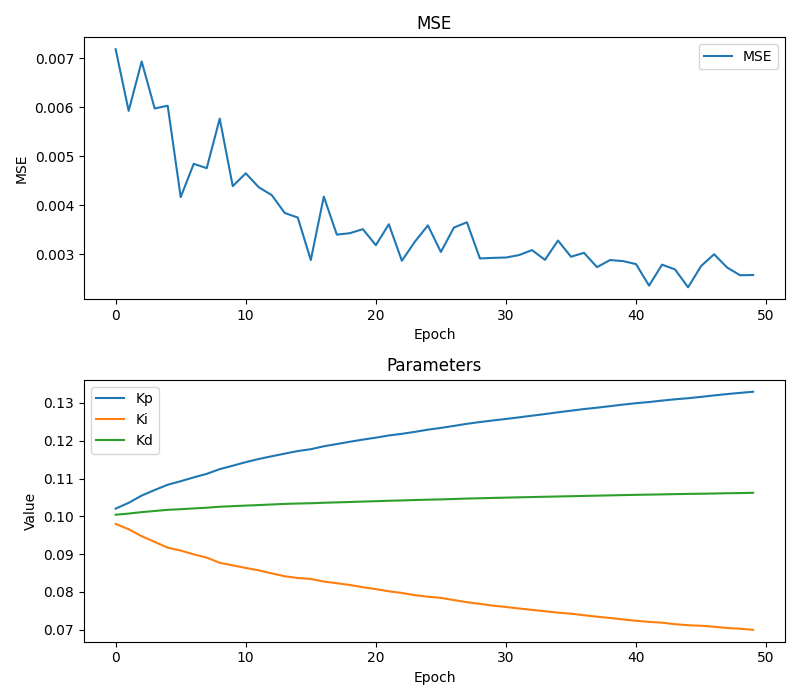
\includegraphics[width=0.8\linewidth]{figures/cournot-classic.png}
\end{center}

For this run we are using a slightly lower disturbance range. This is because the plant was more sensitive, caused
by the lower numbers as input and used as state variables in the plant. The MSE plot indicates a lot of disturbance since
it is not monotonous. The parameter tuning indicates that the $K_i$ is initially too high, and it seems like in this plant
it is more important to consider current error and the differentiation of error instead of the past error history.

\section*{Cournot Plant - AI Controller}

\begin{tabular}{|l|l|}
    \hline
    \textbf{Parameter}   & \textbf{Value}\\ \hline
    Epochs               & 30            \\ \hline
    Timesteps            & 30            \\ \hline
    Learning Rate        & 0.0001          \\ \hline
    Disturbance Range    & (-0.02, 0.02) \\ \hline
    Number of Hidden Layers           & 3           \\ \hline
    Neurons per Layer           & [64, 64, 32]           \\ \hline
    Initial Weight/Bias Range           & (-0.001, 0.001)           \\ \hline
    Activation Function                    & relu            \\ \hline
    Maximum Price                    & 3            \\ \hline
    Marginal Cost                    & 0.1           \\ \hline
    Target Profit & 0.55             \\ \hline
    Initial $q_1$ & 0.4             \\ \hline
    Initial $q_2$ & 0.7             \\ \hline
\end{tabular}
    
\begin{center}
    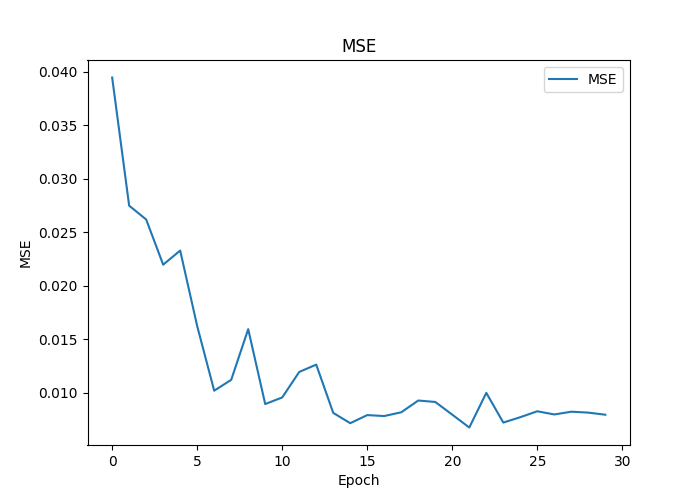
\includegraphics[width=0.8\linewidth]{figures/cournot-ai.png}
\end{center}

The error for this run starts at 0.04. This is a lot higher than 0.007 which is the starting error for the classic
controller when controlling this plant. However, it quickly declines the first 5 epochs, and there is a tendency for declinig
further, but at a slower rate with more disturbances. It performs slightly worse than the classic controller, but it also has
30 epochs instead of 50.

\section*{Population Plant - Classic Controller}

\begin{tabular}{|l|l|}
    \hline
    \textbf{Parameter}   & \textbf{Value}\\ \hline
    Epochs               & 50            \\ \hline
    Timesteps            & 50            \\ \hline
    Learning Rate        & 0.00001          \\ \hline
    Disturbance Range    & (-1, 1) \\ \hline
    Initial $K_p$           & 0.1           \\ \hline
    Initial $K_i$           & 0.1           \\ \hline
    Initial $K_d$           & 0.1           \\ \hline
    Initial Prey Population                    & 90            \\ \hline
    Target Prey Population & 100             \\ \hline
    Initial Predator Population                    & 30           \\ \hline
    Prey Growth Rate & 0.2             \\ \hline
    Predation Rate & 0.01             \\ \hline
    Predator Growth Rate & 0.002             \\ \hline
    Predator Mortality Rate & 0.2             \\ \hline
\end{tabular}

\begin{center}
    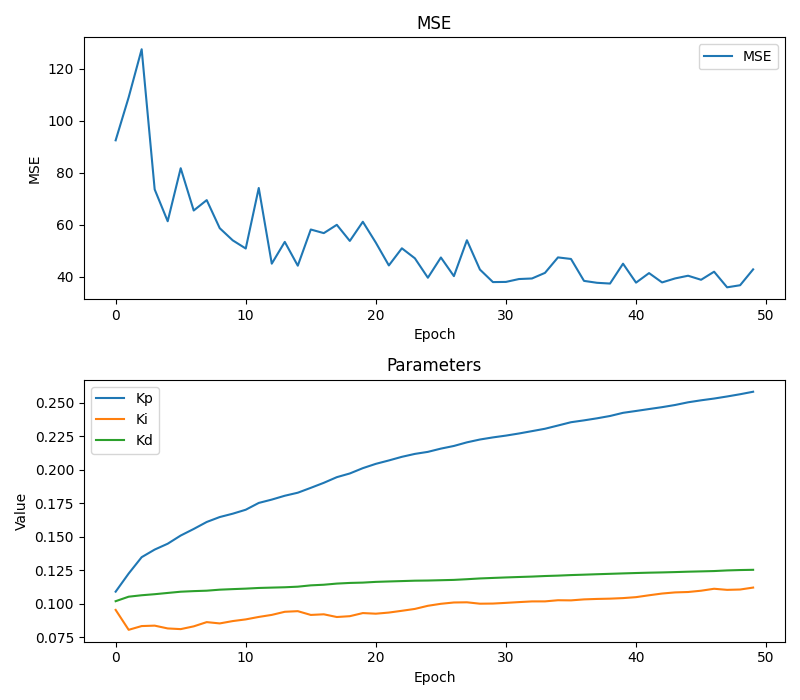
\includegraphics[width=0.8\linewidth]{figures/population-classic.png}
\end{center}

After the first epoch we can see that the error increases. After that it stabilizes again and decrease. There is a lot
of disturbance, and that makes sense given that the mathematical model in this plant is oscilating. The first $K_i$ value
seems to be decreasing too much, and after that it increases. $K_p$ is initially too low.

\section*{Population Plant - AI Controller}

\begin{tabular}{|l|l|}
    \hline
    \textbf{Parameter}   & \textbf{Value}\\ \hline
    Epochs               & 50            \\ \hline
    Timesteps            & 50            \\ \hline
    Learning Rate        & 0.0001          \\ \hline
    Disturbance Range    & (-1, 1) \\ \hline
    Number of Hidden Layers           & 3           \\ \hline
    Neurons per Layer           & [64, 64, 32]           \\ \hline
    Initial Weight/Bias Range           & (-0.1, 0.1)           \\ \hline
    Activation Function                    & relu            \\ \hline
    Initial Prey Population                    & 90            \\ \hline
    Target Prey Population & 100             \\ \hline
    Initial Predator Population                    & 30           \\ \hline
    Prey Growth Rate & 0.2             \\ \hline
    Predation Rate & 0.01             \\ \hline
    Predator Growth Rate & 0.002             \\ \hline
    Predator Mortality Rate & 0.2             \\ \hline
\end{tabular}

\begin{center}
    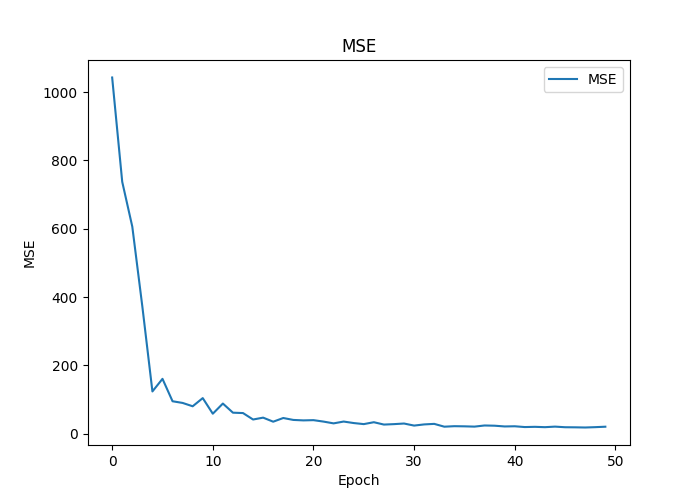
\includegraphics[width=0.8\linewidth]{figures/population-ai.png}
\end{center}

The error is very high after the first epoch. This might be because of the randomly initialized parameters in the neural
network. Error rapidly decreases for the first few epochs. And continue to decrease after that. Better initializing of weights
and biases could lead to a better result. Also when inspecting the gradients it seems like some of the weights are not changed
much.

\clearpage
\section*{Population Plant Description}

This plant is based on Lotka-Volterra equations, which are used to model population oscillations in ecological systems. The basic
idea is that the population of prey and predator will follow each other. When prey population increases, the predator population
will also increase after some time, and vice versa.

The equations are a pair of first order non linear differential equations. 

\begin{align}
    \frac{dx}{dt} &= \alpha x - \beta xy \\
    \frac{dy}{dt} &= \delta xy - \gamma y
\end{align}

Equation 1 is the change in prey population and equation 2 is the change in predator population. $\alpha$ represents the grotwh
rate of prey. $\beta$ represents the preation rate, whihc says something about the effect of predators on prey population.

$\delta$ is the predator growth rate and $\gamma$ is the predator mortality rate.

The solution to these differential equations is the trivial solution when x and y is both 0, and the solutions


\begin{equation}
    \{ y = \frac{\alpha}{\beta}, x = \frac{\gamma}{\delta}\}
\end{equation}

This is the equilibrium state, which means that if x and y is initially set to these values, they will not change.

In our plant we want to control the prey population, so we introduce the control signal $U$ to the change in x.

We also introduce noise to the predator population. Thus the new equations for change in populations become

\begin{align}
    \frac{dx}{dt} &= \alpha x - \beta xy + U \\
    \frac{dy}{dt} &= \delta xy - \gamma y + D
\end{align}


\printbibliography

\end{document}